% =============================================================================
% =============================================================================
% =============================================================================
\section{``Tuna Half'' Dimensional Simulation}
  \label{sec_tuna}

The present section describes the implementation of Tuna, a new two and a half dimensional \Alfven wave code based largely on work by Lysak\cite{lysak_2004,lysak_2013}. 

The half-integer dimensionality refers to the fact that Tuna's spatial grid resolves a two-dimensional slice of the magnetosphere, but that electric and magnetic fields -- as well as their curls -- are three-dimensional vectors. This apparent contradiction is reconciled by the use of a fixed azimuthal modenumber, \azm. Electric and magnetic fields are taken to be complex-valued, varying azimuthally per $\exp\arg{i\azm\phi}$; derivatives with respect to $\phi$ are then replaced by a factor of $i\azm$. 

Unlike a fully three-dimensional code, Tuna cannot resolve the evolution of wave structures in the azimuthal direction. Furthermore, the model does not allow coupling between the dayside and nightside magnetospheres. What Tuna does offer is efficiency. The model's economical geometry allows it to include a realistic Earthward boundary: grid spacing on the order of \SI{10}{\km}, a height-resolved ionospheric conductivity tensor, and even the computation of magnetic field signatures at the ground. Such features are computationally infeasbile for a large global code. 

Tuna was developed with field line resonance in mind. As discussed in \cref{sec_flrs}, such waves are azimuthally localized, minimizing the importance of Tuna's missing half dimension. Moreover, because field line resonances are known to be affected by both the ionosphere and the plasmasphere, a faithful treatment of the inner magnetosphere is a crucial part of studying them numerically. 

Perhaps the most exciting feature of Tuna is its novel driving mechanism: ring current perturbation. Codes similar to Tuna have traditionally been driven using compressional pulses at the outer boundary\cite{lysak_2004,lysak_2013,waters_2008,waters_2013}. This has precluded the investigation of waves with large azimuthal modenumber -- such as giant pulsations -- which are guided, and thus must be driven from within the magnetosphere. 

\todo{The support software -- the driver and the plotter -- are also significant. Do they get mentioned here? Does the Git repository where the code can be accessed get mentioned here? }

%\todo{From Bob's 2013 paper\cite{lysak_2013} (which was also 2.5D): ``The shear \Alfven and compressional fast mode waves can be coupled not only by the Hall conductivity but also by inhomogeneities in the background plasma, which are unavoidable in a realistic magnetosphere [e.g., Lysak and Yoshikawa, 2006\cite{lysak_2006}; Waters et al., 2012\cite{waters_2013}]. This coupling requires a finite wave vector component in the azimuthal direction, i.e., a finite $m$ in the context of the present model. Because of the $\exp \arg{ i m \phi}$ dependence assumed in this model, the coupling from the inhomogeneity enters as an imaginary part of the coupled wave fields with respect to the initial fields, whereas the Hall conductivity appears in phase with the initial fields. Thus, although a fully three-dimensional model can give a more complete picture of wave propagation [e.g., Lysak, 2004\cite{lysak_2004}; Woodroffe and Lysak, 2012\cite{woodroffe_2012}], the present two-dimensional model serves to illustrate the nature of this coupling.''}

%\todo{Past FLR simulations focused on a single mode, didn't account well for the ionosphere, etc. Lee and Lysak 1989, 1990, 1991, Rankin et al 1993, 1995, 1999, Tikhonchuk and Rankin 2000, 2002. }

%Tuna uses megameters, seconds, megacoulombs, and grams as the fundamental units of length, time, charge, and mass respectively. As a result, electric field is measured in \si{\mV/\meter}, magnetic field is measured in \si{\nano\tesla}, and Poynting flux is measured in \si{\mW/\meter\squared}. The electric constant is expressed in \si{\milli\farad/\meter}, not in units of \ez, not that it really matters. 

% -----------------------------------------------------------------------------
% -----------------------------------------------------------------------------
% -----------------------------------------------------------------------------
\subsection{Physical Parameter Profiles}
  \label{sec_tuna_ionos}

Tuna models Earth's magnetic field to be an ideal dipole:
\begin{align}
  \vec{B}_0 &= \SI{3.1e4}{\nT} \lr{ \frac{R_E}{r} }^3 \lr{ 2 \cos\theta \, \hat{r} - \sin\theta \, \hat{\theta} }
\end{align}

Number density is taken to be the sum of an inverse-radial-dependent auroral profile and a plasmaspheric profile dependent on the $L$-shell\cite{lysak_2013}. 
\begin{align}
  n &= n_{AZ} \frac{ r_{AZ} }{r} + 
  n_{PS} \exp \arg{ \frac{-L}{ L_{PS} } } \lr{ \frac{1}{2} - \frac{1}{2} \tanh \frac{ L - L_{PP} }{ \dL_{PP} } }
\end{align}

Where typical values are $n_{AZ} = \SI{10}{\percc}$ (the number density at the base of the auroral zone), $r_{AZ} = \SI{1}{\RE}$ (the scale height of the auroral density distribution), $n_{PS} = \SI{e4}{\percc}$ (the number density at the base of the plasmasphere), $L_{PS} = \SI{1.1}{\RE}$ (the scale $L$ of the plasmasphere), $L_{PP} = 4$ (the $L$ value of the plasmapause), and $\dL_{PP} = 0.1$ (the thickness of the plasmapause, in $L$). 

The perpendicular component of the electric tensor, \ep, is computed based on Kelley's\cite{kelley_1989} tabulated low-density values, $\epsilon_K$, which are adjusted to take into account the effects of high density in the plasmapause. 
\begin{align}
  \ep &= \epsilon_K + \frac{M n}{B_0^2}
\end{align}

Where $M$ is the mean molecular mass, which is large (\about\SI{28}{\amu}) at \SI{100}{\km} altitude, then drops quickly (down to \SI{1}{\amu} by \about\SI{1000}{\km})\cite{lysak_2013}. 

The \Alfven speed profile is computed from the perpendicular electric constant in the usual way, $\va^2 \equiv \frac{1}{\mz \ep}$. This form takes into account the effect of the displacement current, which becomes important in regions where the \Alfven speed approaches the speed of light. 

While the density profile is held constant for all runs discussed in the present work, the \Alfven speed profile is not. Four different for the low-density perpendicular electric constant $\epsilon_K$, corresponding to the differing ionospheric conditions between the dayside and the nightside, and between the high and low points in the solar cycle. These differences are visible in \cref{fig_va}, particularly in the size of the ionospheric \Alfven resonator (the peak in \Alfven speed in the high-latitude ionosphere). 

\begin{figure}[!htb]
    \centering
    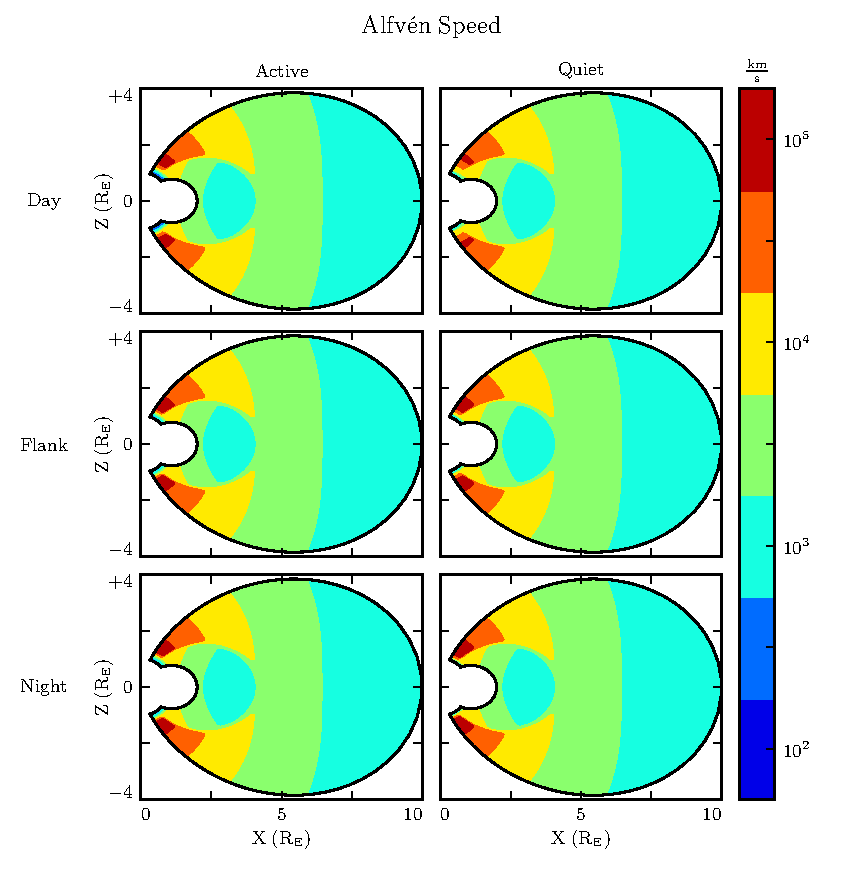
\includegraphics[width=\textwidth]{figures/va.pdf}
    \caption[\Alfven Speed Profiles]{
      \Alfven speed profiles, adapted by Lysak\cite{lysak_2013} from Appendix B of Kelley's textbook\cite{kelley_1989}. 
    }
    \label{fig_va}
\end{figure}

Ionospheric conductivity profiles are also based on values tabulated by Kelley, adjusted by Lysak\cite{lysak_2013} to take into account the abundance of heavy ions near the Earthward boundary. Pedersen, Hall, and parallel conductivities are each resolved by altitude, as shown in \cref{fig_sigma}. 

\begin{figure}[!htb]
    \centering
    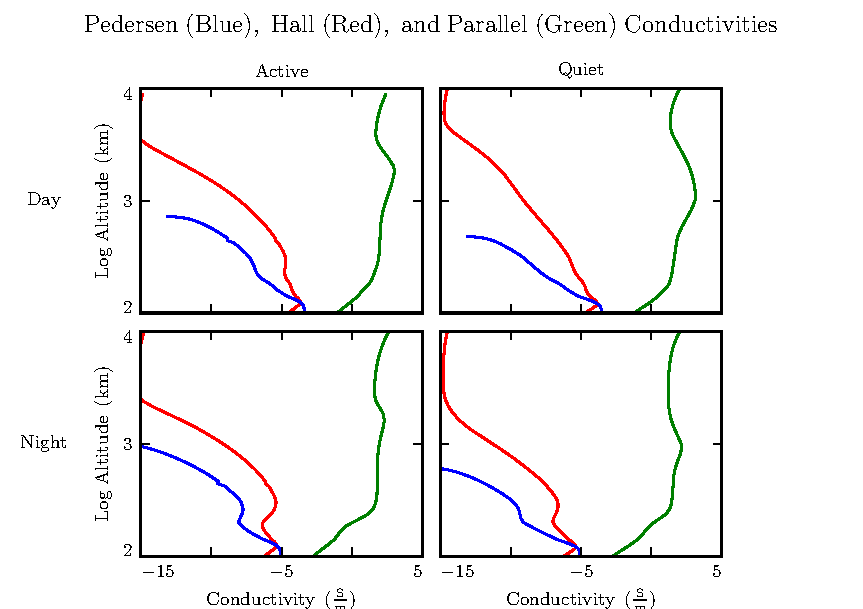
\includegraphics[width=\textwidth]{figures/sigma.pdf}
    \caption[Ionospheric Conductivity Profiles]{
      Ionospheric conductivity profiles, adapted by Lysak\cite{lysak_2013} from Appendix B of Kelley's textbook\cite{kelley_1989}. These profiles allow Tuna to simulate the magnetosphere's response under a variety of conditions. 
    }
    \label{fig_sigma}
\end{figure}

Tuna's physical parameter profiles are static over the course of each run. Even so-called ultra low frequency waves like Pc4 pulsations are fast compared to convective timescales in the magnetosphere. 

%Tuna uses static\footnote{Even so-called ultra low frequency waves like Pc4 pulsations evolve very quickly compared to convective timescales in the magnetosphere. }, height-resolved profiles for the electric tensor and the conductivity tensor. Values are based on those found in Appendix B of Kelley\cite{kelley_1989}, and have been adapted\cite{lysak_2013} to take into account the effects of the plasmasphere. Ionospheric profiles are used to distinguish the dayside magnetosphere from the nightside, and times of high solar activity from quiet times. Conductivity profiles are shown in \cref{fig_sigma}; the \Alfven speed profile is shown in \cref{fig_va}.  

% -----------------------------------------------------------------------------
% -----------------------------------------------------------------------------
% -----------------------------------------------------------------------------
\subsection{Coordinate System}
  \label{sec_coords}

%\todo{Past work which could be cited for geometry examples: Radoski 1967, Lee and Lysak 1989, 1991, Rankin et al 1993, 1994, Streltsov and Lotko 1995, 1999. }

Field line resonance has traditionally been modeled by straightening the field lines into a rectangular configuration\cite{dungey_1954,mann_1995}, by unrolling the azimuthal coordinate into a cylindrical coordinate system\cite{radoski_1974}, or through the use of dipole coordinates\cite{radoski_1967_coords}\footnote{The dipole coordinates \radx, \rady\ and \radz are perhaps more commonly named $\mu$, $\phi$, and $\nu$ respectively; however, in the present work, $\mu$ and $\nu$ take other meanings.}:
\begin{align}
  \label{radoski_coords}
  \radx &\equiv -\frac{\sin^2 \theta}{r} &
  \rady &\equiv \phi &
  \radz &\equiv \frac{\cos \theta}{r^2}
\end{align}

Where $r$, $\theta$, and $\phi$ take on their usual spherical meanings of radial distance, colatitude, and azimuthal angle respectively. 

The dipole coordinate \radx is constant over each equipotential shell\footnote{In fact, \radx is inversely proportional to the McIlwain parameter.}, \rady is azimuthal angle, and \radz indexes each field line from south to north. The unit vectors \xhat, \yhat, and \zhat point in the crosswise\footnote{In the context of in situ measurements taken near the equatorial plane, \xhat is referred to as the radial direction; however, the present work extends the dipole grid to low altitudes, where \xhat can be more horizontal than vertical. The term ``crosswise'' is meant to indicate that \xhat is defined by the cross product of \yhat and \zhat.} (radially outward at the equator), azimuthal (eastward), and parallel (northward at the equator) directions respectively. 

Notably, the dipole coordinates in \cref{radoski_coords} are normal to one another. While mathematically convenient, they do not readily accommodate a fixed-altitude boundary at the ionosphere, nor do they allow the dipole magnetic field to intersect the boundary at an oblique angle, as Earth's field does. As a solution, a nonorthogonal set of dipole coordinates was developed numerically by Proehl\cite{proehl_2002}, then formalized analytically by Lysak\cite{lysak_2004} in terms of their contravariant components:
\begin{align}
  \label{def_coords}
  \lysakx & = - \frac{R_I}{r} \sin^2 \theta & 
  \lysaky & = \phi &
  \lysakz & = \frac{R_I^2}{r^2} \frac{\cos \theta}{\cos \theta_0}
\end{align}

Above, $R_I$ is the position of the ionosphere relative to Earth's center; it's typically taken to be $\SI{1}{\RE} + \SI{100}{\km}$. 

Like the dipole coordinates \radx, \rady, and \radz, Lysak's coordinates \lysakx, \lysaky, and \lysakz correspond to $L$-shell, azimuthal angle, and position along a field line respectively. However, compared to \radz, \lysakz has been renormalized using the invariant colatitude\footnote{The invariant colatitude is the colatitude $\theta$ at which a field line intersects the ionosphere. It is related to the McIlwain parameter by $\cos\theta_0 \equiv \sqrt{1 - \frac{R_I}{L}}$. } $\theta_0$. As a result, \lysakz takes the value \num[retain-explicit-plus]{+1} at the northern ionospheric boundary and \num{-1} at the southern ionospheric boundary for all field lines. 

Because Lysak's coordinate system is not orthogonal\footnote{Curves of constant \lysakx and curves of constant \lysakz can intersect at non-right angles. }, it's necessary to consider covariant and contravariant basis vectors separately. 
\begin{align}
  \hat{e}_i & \equiv \dd{\lysaki} \vec{r} &
  \hat{e}^i & \equiv \dd{ \vec{r} } \lysaki
\end{align}

Covariant basis vectors $\hat{e}_i$ are normal to the curve defined by constant $\lysaki$, while contravariant basis vectors $\hat{e}^i$ are tangent to the coordinate curve (equivalently, $\hat{e}^i$ is normal to the plane defined by constant $u^j$ for all $j \ne i$). These vectors are reciprocal\footnote{The symbol $\delta^i_j$ is the Kronecker delta; the present work also makes use of the Levi-Civita symbol $\varepsilon^{ijk}$ and Einstein's convention of implied summation over repeated indeces\cite{einstein_1916}. } to one another, and can be combined to give components of the metric tensor $\tensor{g}$\cite{dhaeseleer_1991}. 
\begin{align}
  \label{def_metric}
  \hat{e}^i \cdot \hat{e}_j &= \delta^i_j &
  g_{ij} &\equiv \hat{e}_i \cdot \hat{e}_j &
  g^{ij} &\equiv \hat{e}^i \cdot \hat{e}^j 
\end{align}

The metric tensor allows rotation between covariant and contravariant representations of vectors. 
\begin{align}
  \label{metric}
  A_i &= g_{ij} A^j &
  & \text{and} &
  A^i &= g^{ij} A_j &
  & \text{where} &
  A_i &\equiv \vec{A} \cdot \hat{e}_i &
  & \text{and} &
  A^i &\equiv \vec{A} \cdot \hat{e}^i
\end{align}

In addition, the determinant of the metric tensor is used to define cross products and curls\footnote{The square root of the determinant of the metric tensor is called the Jacobian. It's sometimes denoted using the letter $J$, which the present work reserves for current.}. 
\begin{align}
  \label{jacobian}
  \lr{ \vec{A} \times \vec{B} }^i &= \frac{ \varepsilon^{ijk} }{\jac} A_j B_k &
  & \text{and} &
  \lr{ \curl{A} }^i &= \frac{ \varepsilon^{ijk} }{\jac} \dd{\lysakj} A_k &
  & \text{where} &
  g \equiv \det \tensor{g}
\end{align}

Explicit forms of the basis vectors and metric tensor can be found in the appendix of Lysak's 2004 paper\cite{lysak_2004}. At present, it's sufficient to note the mapping between Lysak's basis vectors and the usual dipole unit vectors\footnote{\todo{Do these need to be written out? Referring people to the code, which will be in a public Git repository, is also a possibility. }}. 
\begin{align}
  \label{def_xyz_directions}
  \xhat &= \frac{1}{ \sqrt{ g^{11} } } \hat{e}^1 &
  \yhat &= \frac{1}{ \sqrt{ g^{22} } } \hat{e}^2 &
  \zhat &= \frac{1}{ \sqrt{ g_{33} } } \hat{e}_3
\end{align}

The basis vectors can also be mapped to the spherical unit vectors, though \cref{def_rqf_directions} is valid only at the ionospheric boundary. 
\begin{align}
  \label{def_rqf_directions}
  \qhat &= \frac{1}{ \sqrt{ g_{11} } } \hat{e}_1 &
  \fhat &= \frac{1}{ \sqrt{ g_{22} } } \hat{e}_2 &
  \rhat &= \frac{1}{ \sqrt{ g^{33} } } \hat{e}^3
\end{align}

The coordinates converge at the equatorial ionosphere, so an inner boundary is necessary to maintain finite grid spacing. It's typically placed at $L=2$. The outer boundary is at $L=10$. The dipole approximation of Earth's magnetic field is tenuous at the outer boundary (particularly on the dayside); however, in practice, wave activity is localized inside $L\sim7$. The grid is spaced uniformly in \lysakx, which gives finer resolution close to Earth and coarser resolution at large distances. 

Spacing in \lysakz is set by placing grid points along the outermost field line. The points are closest together at the ionosphere, and grow towards the equator. The spacing increases in a geometric fashion, typically by \SI{3}{\percent}. 

Typically, Tuna uses a grid 150 points in \lysakx by 350 points in \lysakz. The result is a resolution on the order of \SI{10}{\km} at the ionosphere, which increases to the order of \SI{e3}{\km} at the midpoint of the outermost field line. 

There are no grid points in \lysaky due to the two-and-a-half-dimensional nature of the model. Fields are assumed to vary as $\exp \arg{i \azm \lysaky}$, so derivatives with respect to \lysaky are equivalent to a factor of $i \azm$. In effect, this means that the real component of each field is azimuthally in phase with the (purely real) driving, while imaginary values represent behavior that is azimuthally offset. 

\begin{figure}[!htb]
    \centering
    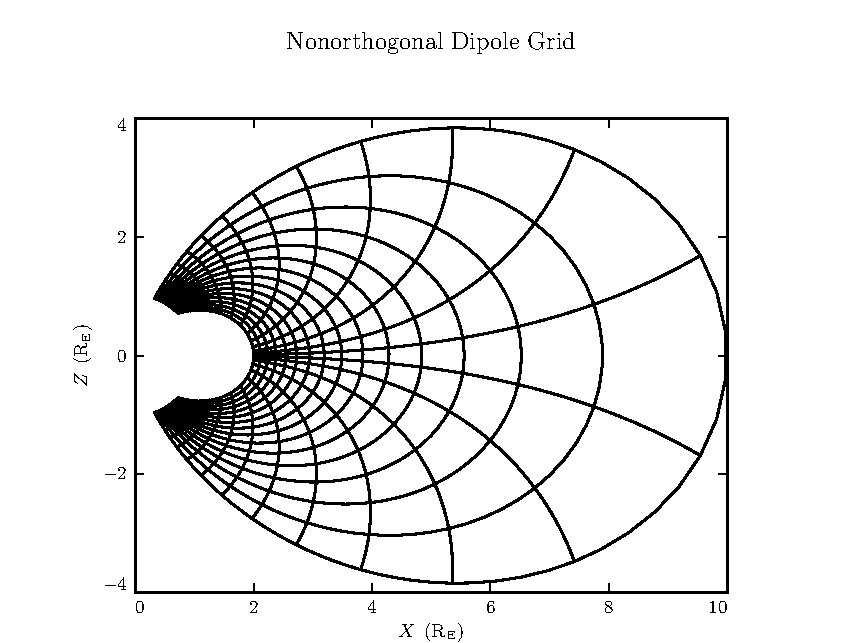
\includegraphics[width=\textwidth]{figures/grid.pdf}
    \caption[Nonorthogonal Dipole Grid]{
      The model's nonorthorthogonal dipole grid. Every fifth point is shown in each direction. The high concentration of grid points near Earth's equator is a consequence of the coordinate system, which converges at the equatorial ionosphere. 
    }
    \label{fig_grid}
\end{figure}

The simulation's time step is set based on the grid spacing. As is the convention, \dt is set to match the smallest \Alfven zone crossing time, scaled down by a Courant factor (typically 0.1). It bears noting that the smallest crossing time need not correspond to the smallest zone; the \Alfven speed peaks several thousand kilometers above Earth's surface, in the so-called Ionospheric \Alfven Resonator\cite{lysak_2013}. A typical time step is on the order of \SI{e-5}{\second}. 

% -----------------------------------------------------------------------------
% -----------------------------------------------------------------------------
% -----------------------------------------------------------------------------
\subsection{Driving}
  \label{sec_driving}

%\todo{This model allows arbitrary driving/propagating waveform, absorption, refraction, phase/group delay, frequency shift, polarization, faraday rotation\cite{simpson_2004,samimi_2015}. }

Models similar to Tuna have traditionally been driven using compression at the outer boundary\cite{lysak_2004,lysak_2013,waters_2008,waters_2013}. Such driving can be envisioned as a proxy for solar wind compression, Kelvin-Helmholtz effects at the magnetopause, and so on. However, because of the constraints imposed by the dispersion relation for \Alfven waves\footnote{See \cref{sec_implications}. }, simulations driven from the outer boundary are constrained to the consideration of waves with low azimuthal modenumber (equivalently, large azimuthal wavelength). 

This issue is demonstrated in \cref{fig_bdrive}. At low modenumber, energy delivered at the outer boundary is able to propagate across field lines in order to stimulate resonances in the inner magnetosphere. However, as modenumber increases, \Alfven waves become increasingly guided, and the inner magnetosphere is unaffected by perturbations at the outer boundary. 

\begin{figure}[!htb]
    \centering
    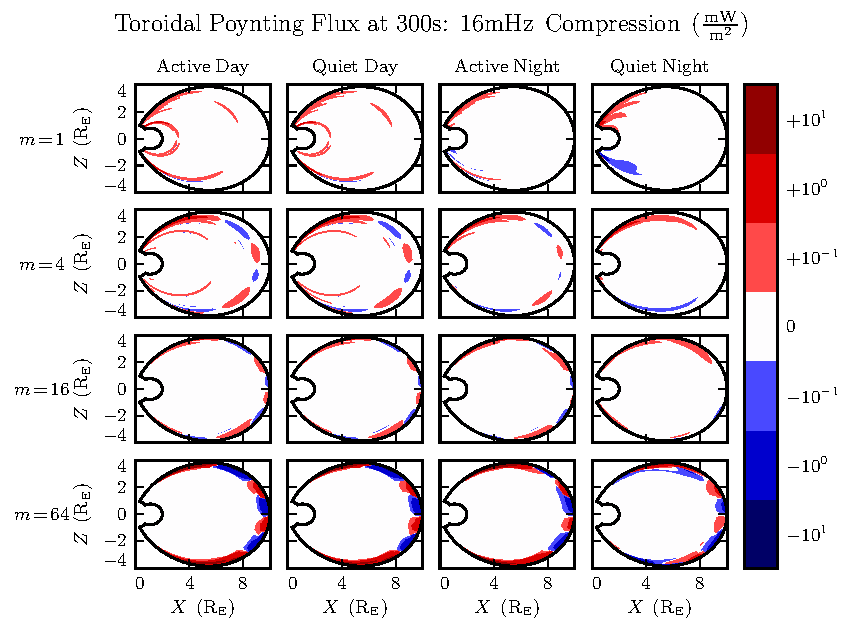
\includegraphics[width=\textwidth]{figures/bdrive.pdf}
    \caption[Decreasing Penetration with Increasing Modenumber]{
      Each cell presents the mean energy density over the course of a \SI{300}{\s} run, as a function of position, due to compressional driving at the outer boundary. Azimuthal modenumber varies by row, and ionospheric conditions vary by column. For runs with small azimuthal modenumber, it's clear that energy is able to propagate across field lines and stimulate wave activity in the inner magnetosphere. When the modenumber is large, energy is unable to penetrate to the inner magnetosphere. Notably, the large values on the bottom row should be taken with a grain of salt; it's not clear that the model's results are reliable when waves are continuously forced against the boundary. 
    }
    \label{fig_bdrive}
\end{figure}

In order to simulate high-modenumber \Alfven waves in the inner magnetosphere -- such as giant pulsations -- a new driving mechanism is necessary. Perturbation of the ring current is a natural choice, as \Alfven waves in the Pc4 range are known to interact with ring current particles through drift and drift-bounce resonances. The ring current is a dynamic region, particularly during and after geomagnetic storms; it's easy to imagine the formation of localized inhomogeneities. 

In order to estimate an appropriate magnitude for perturbations of the ring current, the Sym-H storm index is used. The index is measured once per minute, and so cannot directly detect ring current modulations in the Pc4 frequency range. Instead, the index is transformed into the frequency domain, allowing a fit of its pink noise\footnote{Pink noise, also called $\frac{1}{f}$ noise, refers to the power law decay present in the Fourier transforms of all manner of physical signals. }. 

As shown in \cref{fig_symh}, a Fourier transform of the Sym-H index (taken here from the June 2013 storm) suggests that magnetic field perturbations at Earth's surface due to ring current activity in the Pc4 frequency range could be up to the order of \SI{e-2}{\nT}. Supposing that the ring current is centered around \SI{5}{\RE} geocentric, that corresponds to a current on the order of \SI{0.1}{\mega\ampere}. Tuna's driving is spread using a Gaussian profile in \lysakx (typically centered at $L=5$) and \lysakz (typically centered just off the equator), with a characteristic area of \SI{1}{\RE}$^2$; this gives a current density on the order of \SI{e-4}{\uA/\meter\squared}. 

\todo{Admittedly, estimating the strength of localized perturbations using Sym-H -- an index averaged over the entire globe -- is a bit of a kludge. }

% Note: Not sure why \squared is allowed in some \SI calls but not others... \SI{1}{\RE\squared} throws a \sigma_P in between the R_E and the ^2. For now, we just circumvent the issue. 

\begin{figure}[!htb]
    \centering
    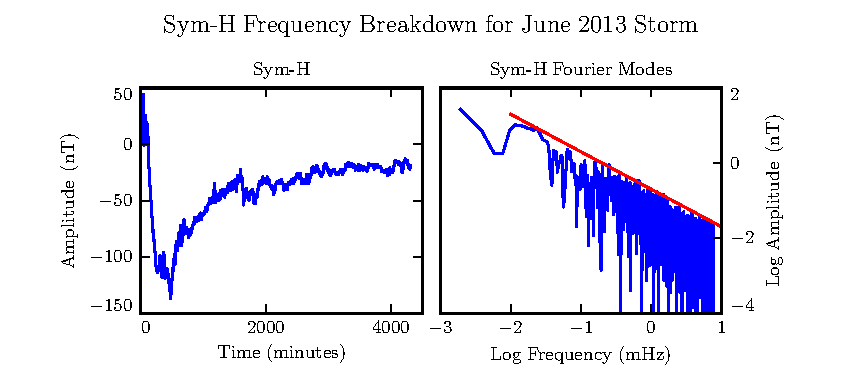
\includegraphics[width=\textwidth]{figures/symh.pdf}
    \caption[Sym-H for June 2013 Storm]{
      The Sym-H storm index\cite{nasa_cdaweb} measures magnetic perturbations on Earth's surface due to ring current activity. The amplitude of oscillations in the Pc4 range is estimated by fitting the pink noise in its Fourier transform. 
    }
    \label{fig_symh}
\end{figure}

In situ observations of Pc4 pulsations and giant pulsations have shown waves with modenumbers across the range $1 \lesssim \azm \lesssim 100$\cite{dai_2013,dai_2015,takahashi_2013}. Simulations are carried out across that range, corresponding to ring current perturbations with azimuthal extent as small as \SI{0.5}{\RE}. 

\todo{Driving is sinusoidal. }

\todo{In case it's not clear: \cref{ch_results} discusses ONLY simulations using ring current driving. The only compressional driving we look at is \cref{fig_bdrive}. }

% -----------------------------------------------------------------------------
% -----------------------------------------------------------------------------
% -----------------------------------------------------------------------------
\subsection{Maxwell's Equations}
  \label{sec_eqns}

% OpenMP. This doesn't really fit. Is it important enough to mention somewhere? Or is this just part of how coding works? 

Tuna simulates the evolution of electromagnetic waves in accordance with \amplaw and \farlaw. Computation is carried out on a Yee grid\cite{yee_1966}: electric fields and magnetic fields are offset by half a time step, and each field component is defined on either odd or even grid points in each dimension to ensure that curls are computed using centered differences. 

%\todo{Leapfrog grid (for which Waters\cite{waters_2013} cites Taflove and Hagness, an electrodynamics textbook). Talk about the grid parity as well as the offset in time. }

%Field values are offset to ensure that most differences are centered. For example, $\ddt B_2$ depends on $\dd{\lysakx} E_3$ and $\dd{\lysakz} E_1$. If $B_2$ is defined at even $i$, $E_3$ is defined at odd $i$, so that $B_2$ is defined on the same grid points as $\frac{ E_3 \lrb{i+1} - E_3 \lrb{i-1} }{ \lysakx \lrb{i+1} - \lysakx \lrb{i-1} }$. 

%\todo{Make sure the example uses the currect parities. }

%Values are sometimes needed off-parity. $E_1$ and $E_2$ are not defined at the same grid locations, but they are coupled directly by the Hall conductivity. And $B_1$ and $B_3$ are coupled by the non-orthogonality of the grid. When off-parity values are needed, they are interpolated from their neighbors. 

%Differentiation and interpolation are good to second order on the nonuniform grid. Like the coefficients for Maxwell's equations, differentiation and interpolation weights are computed during setup to save time during iteration. 

The Ohmic current in \amplaw is replaced with $\; \tensor{\sigma} \cdot \vec{E}\; $ per Kirchhoff's formulation of \ohmlaw. Then, taking \vec{J} to represent the driving current discussed in \cref{sec_driving}, Maxwell's equations can be written 
\begin{align}
  \label{def_eqns}
  \ddt \vec{B} &= - \curl{E} &
  \tensor{\epsilon} \cdot \ddt \vec{E} &= \frac{1}{\mu_0} \curl{B} - \vec{J} - \tensor{\sigma} \cdot \vec{E}
\end{align}

It is convenient to introduce shorthand for the curl of each field: $\vec{C} \equiv \curl{E}$ and $\vec{F} \equiv \curl{B} - \mz \vec{J}$. Or, recalling \cref{jacobian}, 
\begin{align}
  \label{def_curls}
  C^i & = \frac{ \varepsilon^{ijk} }{\jac} \dd{\lysakj} E_k &
  F^i & = \frac{ \varepsilon^{ijk} }{\jac} \dd{\lysakj} B_k - J^i
\end{align}

In these terms, \farlaw can simply be written:
\begin{align}
  \label{farlaw_ijk}
  \ddt B^i &= - C^i
\end{align}

Writing each component out explicitly, and using the metric tensor (per \cref{metric}) to eliminate contravariant magnetic field components\footnote{Fields are stored only in terms of their covariant components, and curls in terms of their contravariant components. This reduces Tuna's memory footprint (since each field need not be stored twice) as well as its computational cost (since time need not be spent rotating between bases). As a result, Tuna's solutions to Maxwell's equations are linear expressions whose coefficients are a mishmash of physical constants and geometric factors. To save time, each coefficient is computed once and stored, rather than being multiplied out from scratch with each time step. }, \cref{farlaw_ijk} becomes:
\begin{align}
  \label{farlaw_final}
  \begin{split}
  B_1 &\assign B_1 - g_{11} \, \dt \, C^1 - g_{13} \, \dt \, C^3 \\
  B_2 &\assign B_2 - g_{22} \, \dt \, C^2 \\
  B_3 &\assign B_3 - g_{31} \, \dt \, C^1 - g_{33} \, \dt \, C^3
  \end{split}
\end{align}

Note that the \assign operator is used in \cref{farlaw_final} to indicate assignment, rather than equality. Terms on the left are new, while those on the right are old. 

Unlike \farlaw, \amplaw cannot be trivially solved. Not only does the derivative of \vec{E} depend on its own future value, but the crosswise and azimuthal components of the equation are coupled by the Hall terms in the conductivity tensor. Fortunately, the electric tensor can be inverted, allowing a solution by integrating factors:
\begin{align}
  \label{int_fac_0}
  \tensor{\epsilon} \cdot \ddt \vec{E} &= \frac{1}{\mu_0} \vec{F} - \tensor{\sigma} \cdot \vec{E} &
  & \text{becomes} &
  \lr{ \tensor{\Omega} + \tensor{ \mathbb{I} } \ddt } \cdot \vec{E} &= \tensor{V}^2 \cdot \vec{F}
\end{align}

Where $\tensor{ \mathbb{I} }$ is the identity tensor and in \x-\y-\z coordinates\footnote{Note the parallel component of the present definition of $\tensor{\Omega}$ differs slightly from that used in \cref{sec_math}.}, 
\begin{align}
  \tensor{V}^2 &\equiv \frac{1}{\mz} \tensor{\epsilon}^{-1} = 
    \mmm{\va^2}{0}{0}
        {0}{\va^2}{0}
        {0}{0}{c^2}
  && \text{and} &
  \tensor{\Omega} &\equiv \tensor{\epsilon}^{-1} \cdot \tensor{\sigma} = 
    \mmm{ \frac{\sp}{\ep} }{ \frac{-\sh}{\ep} }{0}
        { \frac{\sh}{\ep} }{ \frac{\sp}{\ep} }{0}
        {0}{0}{ \frac{\sz}{\ez} } 
\end{align}

Multiplying through by $\exp \arg{ \tensor{\Omega} \, t }$ and applying the product rule, \cref{int_fac_0} becomes\footnote{Tensor exponentiation is analogous to scalar exponentiation\cite{hall_2015}: $\exp \arg{ \tensor{T} } \equiv \displaystyle\sum_n \frac{1}{ n! } \tensor{T}^n$. }
\begin{align}
  \label{int_fac_1}
  \ddt \Big( \exp \arg{\tensor{\Omega} \, t} \cdot \vec{E} \, \Big) &= \exp \arg{\tensor{\Omega} \, t} \cdot \vec{V}^2 \cdot \vec{F}
\end{align}

\cref{int_fac_1} can then be integrated over a small time step \dt and expressed in terms of the assignment operator introduced in \cref{farlaw_ijk}. 
\begin{align}
  \label{int_fac_2}
  \vec{E} &\assign \exp \arg{ -\tensor{\Omega} \, \dt } \cdot \vec{E} + \dt \, \exp \arg{ -\tensor{\Omega} \, \tfrac{\dt}{2} } \cdot \tensor{V}^2 \cdot \vec{F}
\end{align}

The tensor exponential can be evaluated by splitting $\tensor{\Omega}$ into the sum of its diagonal and Hall components
\footnote{For tensors, $\exp \arg{ \tensor{S} + \tensor{T} } = \exp \arg{ \tensor{S} } \exp \arg{ \tensor{T} }$ as long as $\tensor{S} \cdot \tensor{T} = \tensor{T} \cdot \tensor{S}$. }. The Hall exponential condenses into sines and cosines, giving a rotation around the magnetic field line. 
\begin{align}
  \label{amp_final}
  \vec{E} &\assign \exp \arg{ -\tensor{\Omega}' \; \dt } \cdot \tensor{R}_z \arg{ \tfrac{-\sh \dt}{\ep} } \cdot \vec{E}
   + \dt \, \tensor{V}^2 \cdot \exp \arg{ -\tensor{\Omega}' \; \tfrac{\dt}{2} } \cdot \tensor{R}_z \arg{ \tfrac{-\sh \dt}{2 \ep} } \cdot \vec{F}
\end{align}

Where 
\begin{align}
  \tensor{R}_z \arg{\theta} &= 
  \mmm{\cos\theta}{-\sin\theta}{0}
      {\sin\theta}{\cos\theta}{0}
      {0}{0}{1} &
  & \text{and} &
  \tensor{\Omega}' &\equiv
    \mmm{ \frac{\sp}{\ep} }{0}{0}
        {0}{ \frac{\sp}{\ep} }{0}
        {0}{0}{ \frac{\sz}{\ez} }
\end{align}

The parallel component of term of \cref{amp_final} is simply
\begin{align}
  E_z \assign E_z \exp \arg{ \tfrac{- \sz \dt}{\ez} } + c^2 \dt F_z \exp \arg{ \tfrac{- \sz \dt}{2 \ez} }
\end{align}

Or, using \cref{def_xyz_directions} to map to the covariant basis, 
\begin{align}
  \label{e3_final}
  E_3 \assign E_3 \exp \arg{ \tfrac{- \sz \dt}{\ez} } + c^2 \dt \lr{ g_{31} F^1 + g_{33} F^3 } \exp \arg{ \tfrac{- \sz \dt}{2 \ez} }
\end{align}

Tuna's conductivity profile gives a minimum value of $\frac{\sz \dt}{\ez}$ on the order of \num{e3}, making $\exp \arg{ \frac{- \sz \dt}{\ez} }$ far too small to be stored in a double precision variable\footnote{Not coincidentally, $\frac{\sz}{\ez}$ can also be written $\frac{\op^2}{\nu}$. At the ionosphere, the collision frequency $\nu$ is fast compared to field line resonance timescales, but it's still slow compared to the plasma frequency.}. That is, this model takes $E_3$ (and, proportionally, $E_z$) to be uniformly zero. This issue is revisited in \cref{sec_inertia}. 

The perpendicular components of \cref{amp_final} give the expressions: 
\begin{alignat}{6}
  \label{e1_final}
  & E_1 + \frac{ g^{13} }{ g^{11} } && E_3 \assign &&   && E_1 && \cos \arg{ \tfrac{- \sh \dt}{\ep} } \exp \arg{ \tfrac{- \sp \dt}{\ep} } &&  \notag \\
  &                                 &&             && + && E_2 && \sin \arg{ \tfrac{- \sh \dt}{\ep} } \exp \arg{ \tfrac{- \sp \dt}{\ep} } &&  \sqrt{ \frac{ g^{22} }{ g^{11} } } \notag \\
  &                                 &&             && + && E_3 && \cos \arg{ \tfrac{- \sh \dt}{\ep} } \exp \arg{ \tfrac{- \sp \dt}{\ep} } &&  \frac{ g^{13} }{ g^{11} } \\
  &                                 &&             && + && F^1 && \cos \arg{ \tfrac{- \sh \dt}{2\ep} } \exp \arg{ \tfrac{- \sp \dt}{2\ep} } &&  \frac{\va^2 \dt}{ g^{11} } \notag \\
  &                                 &&             && + && F^2 && \sin \arg{ \tfrac{- \sh \dt}{2\ep} } \exp \arg{ \tfrac{- \sp \dt}{2\ep} } &&  \frac{\va^2 \dt}{ \sqrt{ g^{11} g^{22} } } \notag \\
  \intertext{and}
  \label{e2_final}
  & && E_2 \assign && - && E_1 && \sin \arg{ \tfrac{- \sh \dt}{\ep} } \exp \arg{ \tfrac{- \sp \dt}{\ep} } &&  \sqrt{ \frac{ g^{11} }{ g^{22} } } \notag \\
  & &&             && + && E_2 && \cos \arg{ \tfrac{- \sh \dt}{\ep} } \exp \arg{ \tfrac{- \sp \dt}{\ep} } &&  \notag \\
  & &&             && - && E_3 && \sin \arg{ \tfrac{- \sh \dt}{\ep} } \exp \arg{ \tfrac{- \sp \dt}{\ep} } &&  \frac{ g^{13} }{ \sqrt{ g^{11} g^{22} } } \\
  & &&             && - && F^1 && \sin \arg{ \tfrac{- \sh \dt}{2\ep} } \exp \arg{ \tfrac{- \sp \dt}{2\ep} } &&  \frac{\va^2 \dt}{ \sqrt{ g^{11} g^{22} } } \notag \\
  & &&             && + && F^2 && \cos \arg{ \tfrac{- \sh \dt}{2\ep} } \exp \arg{ \tfrac{- \sp \dt}{2\ep} } &&  \frac{\va^2 \dt}{ g^{22} } \notag
\end{alignat}

The $E_3$ terms in \cref{e1_final,e2_final} can be ignored at present. They are revisited in \cref{sec_inertia}. 

% -----------------------------------------------------------------------------
% -----------------------------------------------------------------------------
% -----------------------------------------------------------------------------
\subsection{Boundary Conditions}
  \label{sec_bcs}

%\todo{Some ground signature work as far back as Greifinger and Greifinger in 1968\cite{greifinger_1968}, but there's been steady advancement. Lysak and Song, in 2006, were the first to work out ground signatures without the assumption of a single-frequency wave. }

%\todo{Past work that got ground signatures (without latitude-dependent zenith angle) Greifinger and Greifinger 1968, 1973, Hughes 1974, Sciffer and Waters 2002, Sciffer et al 2005. Better computation of ground signatures... Waters and Sciffer 2008, Sciffer and Waters 2011, Woodroffe and Lysak 2012. }

Dirichlet and Neumann boundary conditions are applied to the electric field components and magnetic field components respectively. That is, electric fields are forced to go to zero at the inner and outer boundaries, and magnetic fields are forced to have a zero derivative normal to the inner and outer boundaries. 

These boundary conditions can in principle cause nonphysical reflections at the boundary\footnote{See, for example, the bottom row of \cref{fig_bdrive}. }. However, in practice, wave activity is concentrated well within the simulation domain. Simulation results are robust under an exchange of Dirichlet and Neumann boundary conditions (though a self-inconsistent set of boundary condidtions, such as applying Neumann boundary conditions to $B_1$ but Dirichlet boundary conditions to $B_3$, quickly causes instability). 

The Earthward boundary conditions are as follows. 

Between the top of the neutral atmosphere and the bottom of the ionosphere, the model includes a thin, horizontal current sheet representing the ionosphere's $E$ layer\cite{lysak_2004}. By integrating \amplaw over the layer, it can be shown\cite{fujita_1988} that the horizontal electric field values at the edge of the grid are determined by the jump in the horizontal magnetic fields:
\begin{align}
  \label{jump_condition}
  \tensor{\Sigma} \cdot \vec{E} &= \frac{1}{\mz} \, \displaystyle\lim_{\dr \rightarrow 0} \, \bigg[ \, \hat{r} \times \vec{B} \, \bigg|^{R_I + \dr}_{R_I - \dr}
\end{align}

The integrated conductivity tensor $\tensor{\Sigma}$ can be written in $\theta$-$\phi$ coordinates as\cite{lysak_2004}:
\begin{align}
  \label{def_sigma}
  \tensor{\Sigma} &\equiv \mm{ \frac{\Sigma_0 \Sigma_P}{ \Sigma_0 \cos^2 \alpha + \Sigma_P \sin^2 \alpha } }{ \frac{-\Sigma_0 \Sigma_H}{ \Sigma_0 \cos^2 \alpha + \Sigma_P \sin^2 \alpha } }
                             { \frac{\Sigma_0 \Sigma_H}{ \Sigma_0 \cos^2 \alpha + \Sigma_P \sin^2 \alpha } }{ \Sigma_P + \frac{\Sigma_H^2 \sin^2 \alpha}{ \Sigma_0 \cos^2 \alpha + \Sigma_P \sin^2 \alpha } } \end{align}

Where $\alpha$ is the angle between the magnetic field and the vertical direction, given by $\cos \alpha \equiv \frac{ -2 \cos \theta }{ \sqrt{1 + 3 \cos^2\theta} }$, and $\Sigma_P$, $\Sigma_H$, and $\Sigma_0$ are the height-integrated Pedersen, Hall, and parallel conductivities respectively. Their values are determined by integrating Kelley's\cite{kelley_1989} conductivity profiles from Earth's surface to the ionospheric boundary; values are shown in \cref{tab_sigma_atm}. 

\begin{longtable}{ @{\extracolsep{\fill}} lrrr @{\extracolsep{\fill}} }
  \caption[Integrated Atmospheric Conductivity]{Integrated Atmospheric Conductivity (\si{\S})}
  \label{tab_sigma_atm} \\
  \toprule
  & $\Sigma_0$ & $\Sigma_P$ & $\Sigma_H$ \\
  \midrule
  \endfirsthead
  \bottomrule
  \endlastfoot
  Active Day   & 424 & 0.65 & 6.03 \\
  Quiet Day    & 284 & 0.44 & 4.02 \\
  Active Night &   9 & 0.01 & 0.12 \\
  Quiet Night  &   9 & 0.01 & 0.12 \\
\end{longtable}

An expression for the horizontal electric fields at the boundary can be obtained by inverting \cref{jump_condition}. After mapping to covariant coordinates per \cref{def_rqf_directions}, and taking $\Sigma \equiv \det \tensor{\Sigma}$,
\begin{align}
  \label{eatm_final}
  \begin{alignedat}{6}
  & E_1 \assign \frac{1}{\mz \Sigma} \, \displaystyle\lim_{\dr \rightarrow 0} \, \bigg[ \, &- & \Sigma_{\theta\phi} && B_1   && - \sqrt{ \frac{ g_{11} }{ g_{22} } }&&\Sigma_{\phi\phi} && B_2 \, \bigg|^{R_I + \dr}_{R_I - \dr} \\
  & E_2 \assign \frac{1}{\mz \Sigma} \, \displaystyle\lim_{\dr \rightarrow 0} \, \bigg[ \, &\sqrt{ \frac{ g_{22} }{ g_{11} } } & \Sigma_{\theta\theta} && B_1 && +  &&\Sigma_{\phi\theta} && B_2 \, \bigg|^{R_I + \dr}_{R_I - \dr}
  \end{alignedat}
\end{align}

The atmospheric magnetic field is computed as a linear combination of harmonics. The neutral atmosphere is considered to be a perfect insulator, giving $\curl{B}=0$. Combined with $\div{B}=0$ (per Maxwell's equations), this allows the computation of a magnetic scalar potential $\Psi$ such that $\vec{B}=\grad{\Psi}$ and $\Psi$ satisfies Laplace's equation, $\nabla^2 \Psi = 0$. 

Laplace's equation can be solved analytically; however, a numerical solution is preferrable to ensure orthonormality on a discrete and incomplete\footnote{As discussed in \cref{sec_coords}, the grid is constrained to finite $L$, which excludes the equator as well as the poles. } grid. After separating out the radial and azimuthal dependence in the usual way, the latitudinal component of Laplace's equation can be written in terms of $s \equiv - \sin^2 \theta$: 
\begin{align}
  \label{laplace}
  \lr{ 4 s^2 + 4s } \frac{d^2}{ds^2} Y_\ell + \lr{ 4 + 6 s } \frac{d}{ds} Y_\ell - \frac{\azm^2}{s} Y_\ell &= \ell \, \lr{ \ell + 1 } Y_\ell
\end{align}

Using centered differences to linearize the derivatives, \cref{laplace} becomes a system of coupled linear equations, one per field line. It can be solved numerically for eigenvalues $\ell \, \lr{\ell + 1}$ and eigenfunctions $Y_\ell$\footnote{Solving Laplace's equation analytically results in spherical harmonics indexed by both $\ell$ and \azm, the separation constants for $\theta$ and $\phi$ respectively. In two and a half dimensions, $\phi$ is not explicitly resolved, so \azm is set manually.}. In terms of the harmonics $Y_\ell$, $\Psi$ between the Earth's surface and the top of the atmosphere can be written
\begin{align}
  \label{psi_expansion}
  \Psi &= \displaystyle\sum_\ell \lr{ a_\ell \, r^\ell + b_\ell \, r^{-\ell - 1} } Y_\ell
%  \Psi \arg{r, \theta} &= \displaystyle\sum_\ell \lr{ a_\ell \, r^\ell + b_\ell \, r^{-\ell - 1} } Y_\ell \arg{\theta}
\end{align}

As a boundary condition for $\Psi$, Earth is assumed to be a perfect conductor. This forces the magnetic field at Earth's surface to be horizontal; that is, $B_r = \dd{r} \Psi = 0$. Noting that solutions to Laplace's equation are orthonormal, each element of the sum in \cref{psi_expansion} must be independently zero at $R_E$. This allows the coefficients $a_\ell$ and $b_\ell$ to be expressed in terms of one another. 
\begin{align}
  \label{beta_solution}
  b_\ell &= \frac{\ell}{\ell + 1} R_E^{2 \ell + 1} a_\ell
\end{align}

The current sheet at the top of the atmosphere is assumed to be horizontal, so the radial component of the magnetic field must be the same just above and just below it. Taking the radial derivative of \cref{psi_expansion} at the top of the atmosphere, and eliminating $b_\ell$ with \cref{beta_solution}, gives
\begin{align}
  B_r &= \displaystyle\sum_\ell \ell \, a_\ell \, R_I^{\ell-1} \, \lr{ 1 - \lambda^{2 \ell + 1} } Y_\ell &
  & \text{where} &
  \lambda &\equiv \frac{R_E}{R_I} \sim \num{0.975}
\end{align}

The summation can be collapsed by ``integrating'' over a harmonic\footnote{Because the functions are defined on a discrete grid, their inner product is not an integral, but a sum: $B_r \cdot Y_\ell^{-1} \equiv \displaystyle\sum_i B_r [i] \; Y_\ell^{-1} \! [i] $. }. Inverse harmonics can be obtained by inverting the eigenvector matrix. Then $Y_\ell \cdot Y_{\ell'}^{-1} = \delta_{\ell \ell'}$ by construction. 
\begin{align}
  \label{alpha_solution}
  a_\ell &= \frac{ 1 }{\ell \, R_I^{\ell-1} } \frac{ B_r \cdot Y_\ell^{-1} }{ 1 - \lambda^{2 \ell + 1} }
\end{align}

Combining \cref{psi_expansion,beta_solution,alpha_solution} allows the expression of $\Psi$ at the top and bottom of the atmosphere as a linear combination of radial magnetic field components at the bottom of the ionosphere. 
\begin{align}
  \label{psi_final}
  \begin{split}
  \Psi_E &= \displaystyle\sum_\ell Y_\ell \; \frac{R_I}{ \ell \, \lr{\ell - 1} } \frac{ \lr{2 \ell - 1} \, \lambda^\ell }{ 1 - \lambda^{2 \ell + 1} } B_r \cdot Y_\ell^{-1} \\
  \Psi_I &= \displaystyle\sum_\ell Y_\ell \; \frac{R_I}{ \ell \, \lr{\ell - 1} } \frac{ \lr{\ell - 1} + \ell \, \lambda^{2 \ell + 1} }{ 1 - \lambda^{2 \ell + 1} } B_r \cdot Y_\ell^{-1}
  \end{split}
\end{align}

Horizontal magnetic fields are obtained by taking derivatives of $\Psi$. 
\begin{align}
  B_1 &= \dd{\lysakx} \Psi &
  B_2 &= \dd{\lysaky} \Psi
\end{align}

Horizontal magnetic field values at the top of the atmosphere are used to impose boundary conditions on the electric fields at the bottom of the ionosphere, per \cref{eatm_final}. Those at Earth's surface are valuable because they allow a direct comparison between model output and ground magnetometer data, after being mapped to physical coordinates per \cref{def_rqf_directions}. 



